% \documentclass[subf, href, colorlinks=true, 14pt,
% times, mtpro, specialist]{disser}

% Base defines -- begin
% \usepackage[
% a4paper, mag=1000, includefoot,
% left=3cm, right=1.5cm, top=2cm, bottom=2cm, headsep=1cm, footskip=1cm
% ]{geometry}
% \usepackage[T2A]{fontenc}
% \usepackage[utf8]{inputenc}
% \usepackage[english, russian]{babel}
% Base defines -- end

% \usepackage{answers}
% \usepackage{graphicx}
% \graphicspath{ {./src/pic/} }
% \usepackage{wrapfig}
%\usepackage[export]{adjustbox}
% \usepackage{appendix}
% \usepackage{multirow}
% \usepackage{multicol}
% \usepackage{mathrsfs,amsmath,amsthm,amssymb}
% \usepackage{verbatim}
% \usepackage{url}
% \usepackage{indentfirst}
% 
% \usepackage{tikz}
% \usetikzlibrary{decorations.pathreplacing}

\documentclass[subf, href, colorlinks=true, 14pt,
times, mtpro, specialist]{disser}

\usepackage[
a4paper, mag=1000, includefoot,
left=3cm, right=1.5cm, top=2cm, bottom=2cm, headsep=1cm, footskip=1cm
]{geometry}
\usepackage[T2A]{fontenc}
\usepackage[utf8]{inputenc}
\usepackage[english, russian]{babel}

\usepackage{answers}
\usepackage{graphicx}
\usepackage{appendix}
\usepackage{multicol}
\usepackage{mathrsfs,amsmath,amsthm,amssymb}
\usepackage{verbatim}
\usepackage{url}

\usepackage{indentfirst}
\usepackage{amsmath}
\usepackage{amssymb}
\usepackage{epstopdf}
\usepackage[usenames, dvipsnames]{color}
\usepackage{colortbl}
\usepackage{amstext}
\usepackage{courier}
\usepackage{float}
\usepackage{wrapfig}

\usepackage{enumitem}

\graphicspath{ {./src/pic/} }

%%%%%%%%%%%%%%%%%%%%%%%%%%%%%%%%%%%%%%%%%%%%%%%%%%%%%%%%%%%%%%%%%%%%%%%%
% Хак с шрифтами
\IfFileExists{pscyr.sty}
{
	\usepackage{times}
	\usepackage{mathptmx}
	\usepackage{pscyr}
	\def\rmdefault{ftm}
	\def\sfdefault{ftx}
	\def\ttdefault{fer}
	
	\DeclareMathAlphabet{\mathbf}{OT1}{ftm}{bx}{it} % bx/it or bx/m
}
{ % else
	\typeout{RFDstyle message: no pScyr, shall do without...}
}
%%%%%%%%%%%%%%%%%%%%%%%%%%%%%%%%%%%%%%%%%%%%%%%%%%%%%%%%%%%%%%%%%%%%%%%%
\newcommand{\figref}[1]{\figurename~\ref{#1}}

\newcommand{\specialcell}[2][c]{%
  \begin{tabular}[#1]{@{}c@{}}#2\end{tabular}}

\def\const{\mathop{\rm const}\nolimits}
\def\Div{\mathop{\rm div}\nolimits}

\theoremstyle{definition}
\newtheorem{defn}{Определение}[section]

\begin{document}
	
	\makeatletter
	
	\newgeometry{includefoot,
		left=3cm, right=1.5cm, top=2cm, bottom=0cm, headsep=1cm, footskip=1cm}
	
	\ifundeflength\firstskip{1.5cm}
	\ifundeflength\secondskip{4.5cm}
	\ifundeflength\thirdskip{3ex}
	\ifundeflength\fourthskip{1ex}
	\ifundeflength\fifthskip{1ex}
	\ifundeflength\sixthskip{2cm}
	\ifundeflength\seventhskip{2ex}
	
	\vskip 2em%
	\thispagestyle{empty}
	\vspace*{-2cm}
	\begin{center}  
		{\instfont\@institution{ФЕДЕРАЛЬНОЕ ГОСУДАРСТВЕННОЕ БЮДЖЕТНОЕ ОБРАЗОВАТЕЛЬНОЕ УЧРЕЖДЕНИЕ ВЫСШЕГО ОБРАЗОВАНИЯ <<МОСКОВСКИЙ ГОСУДАРСТВЕННЫЙ УНИВЕРСИТЕТ \\
				имени М.\,В.\,ЛОМОНОСОВА>> \\
				\vskip\fifthskip
				МЕХАНИКО-МАТЕМАТИЧЕСКИЙ ФАКУЛЬТЕТ \\
				\vskip\fifthskip
				КАФЕДРА ВЫЧИСЛИТЕЛЬНОЙ МАТЕМАТИКИ}}
	\end{center}
	\vskip\firstskip
	\begin{center}
		{\@title{ВЫПУСКНАЯ КВАЛИФИКАЦИОННАЯ РАБОТА \\ 
				(ДИПЛОМНАЯ РАБОТА) СПЕЦИАЛИСТА}}
		\vskip\fifthskip
		{\topicfont\@topic{<<Распределённая система хранения состояния на основе алгоритма для решения задач консенсуса в распределенной среде ненадежных узлов>>}}
		
	\end{center}
	\normalfont
	\vskip\firstskip
	\hfill
	\begin{minipage}{.5\linewidth}
		Выполнил студент {\@group{610 группы}} \\
		{\@author{Федотов Иван Андреевич}}
		\vskip\thirdskip
		\begin{tabular}{ll}
			\makebox[2.5in]{\hrulefill}\\
			подпись студента
		\end{tabular}
		\vskip\thirdskip
		Научный руководитель: \\
		д.\,ф.-м.\,н., профессор {\@sa{К. Ю. Богачев}}
		\vskip\thirdskip
		\begin{tabular}{ll}
			\makebox[2.5in]{\hrulefill}\\
			подпись научного руководителя
		\end{tabular}
	\end{minipage}
	\vfill
	\begin{center}
		{\@city{Москва} \\ \@date}
	\end{center}
	\normalfont
	\restoregeometry
	\clearpage
	
	%
	
	% Включать подсекции в оглавление
	\setcounter{tocdepth}{2}
	
	\tableofcontents
	\pagebreak

%%%%%%%%%%%%%%%%%%%%%%%%%%%%%%%%%%%%%%%%%%%%%%%%%%%%%%%%%%%%%%%%%%%%%%%%%%%%%%%%%%%%%%%%%%%


\section{Постановка задачи}

Распределённая система - это совокупность взаимосвязанных компьютеров или устройств, работающих в сети и совместно выполняющих задачи и обработку данных. В современном мире такие системы играют ключевую роль в обеспечении надёжности, масштабируемости и отказоустойчивости при работе с данными. Однако, управление состоянием в таких системах представляет собой нетривиальную задачу из-за потенциальной ненадежности сети, отказов узлов и асинхронной природы сообщений. Для обеспечения консенсуса в распределённых системах существует множество алгоритмов, каждый из которых имеет свои преимущества и недостатки. В данной дипломной работе будет проведено исследование алгоритмов консенсуса с целью их использования для построения распределённых систем.

Основной задачей данной дипломной работы является реализация на языке C++ программы, создания распределённой системы на основе одного из алгоритмов консенсуса, и дальнейшее использование этой программы на существующей централизованной системе для построения распределённой системы на её основе.
Внедрение алгоритма консенсуса в такую систему позволит значительно повысить надежность и отказоустойчивость, а также добавит возможность её масштабирования. 

В ходе исследования, подробности которого будут представлены далее, для реализации распределённой системы был выбран алгоритм Raft. Этот алгоритм является понятным, легко поддающимся внедрению и обладающим высокой степенью устойчивости к различным сбоям. Работа с данным алгоритмом представляет интерес как с точки зрения теоретических аспектов, так и с практической стороны, позволяя изучить процесс адаптации и интеграции алгоритма в уже действующую систему.

\section{Введение}

Определим основные понятия, используемые далее.
\begin{itemize}
\item \emph{Распределенная система} - это набор независимых компьютеров (\emph{узлов}), которые представляются пользователю как единая согласованная система.

\begin{figure}[H]
\label{fig:dist_sys}
\centering
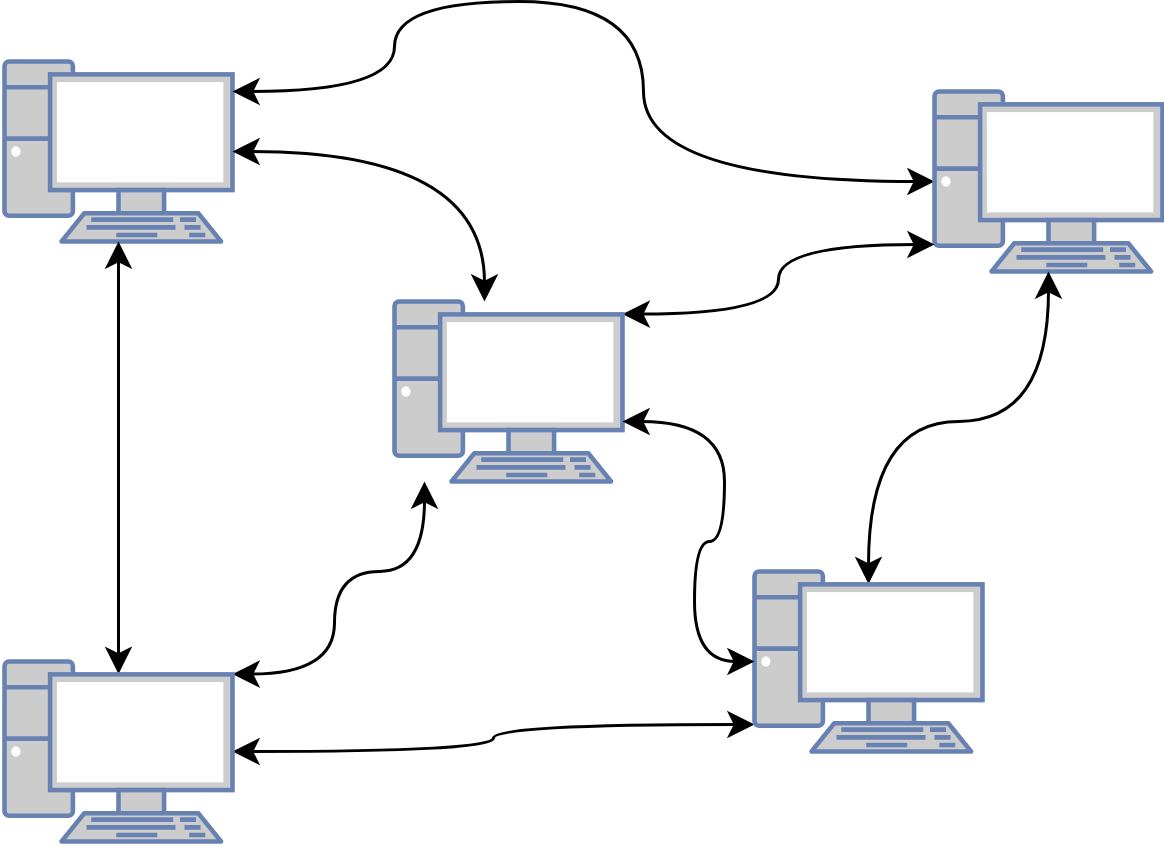
\includegraphics[width=0.6\textwidth]{src/pics/dist_sys.png}
\caption{Распределённая система.}
\end{figure}

\item \emph{Задача достижения консенсуса} - это задача получения согласованного значения группой участников, члены которой называются \emph{узлами}, в ситуации, когда возможны отказы отдельных участников, предоставления им некорректной информации или искажения переданных значений средой передачи данных.
\end{itemize}



\subsection{Описание задачи принятия консенсуса}

Как уже упоминалось, задача принятия консенсуса является одной из основополагающих для современных распределенных компьютерных систем. 

Консенсус должен удовлетворять следующим условиям:
\begin{enumerate}
\item \textbf{Согласованность}: все корректные работающие узлы принимают одно и то же значение (\textit{"свойство безопасности"});
\item \textbf{Корректность}: выбранное значение должно быть одним из тех, которое было предложено каким-либо корректно работающим узлом (\textit{"свойство нетривиальности"});
\item \textbf{Конечность}: каждый корректно работающий узел должен делать выбор за конечное количество шагов (\textit{"свойство завершённости"});
\end{enumerate}

Теорема Фишера, Линча и Патерсона гласит, что не существует асинхронного детерминированного алгоритма принятия консенсуса, который был бы устойчив к выходу из строя одного узла и гарантировал бы все свойства консенсуса \cite{Theorem_FLP}. Асинхронизм означает, что нельзя достоверно различить работает ли узел медленно, или долго идет сообщение, или же отказал узел, даже если предположить, что связь является надежной. Алгоритм Raft гарантирует только свойство безопасности (1) и нетривиальности (2), но не всегда удовлетворяют свойству завершенности (3).

\subsection{Возможные типы ошибок}

В контексте задачи консенсуса существуют разные типы ошибок:
\begin{enumerate}
\item \textbf{Остановка с сигналом}: узел прекращает работу, а затем сообщает другим узлам о своем сбое. Этот тип ошибки позволяет точно определить, отказал ли узел или нет; такие ошибки предоставляют самые удобные для реализации предположения относительно сбоев в системе;

\item \textbf{Остановка}: узел преждевременно прекращает какую-либо активность, несмотря на то, что до остановки он работал полностью корректно. Предполагается, что узел может восстанавливается после остановки и включается в работу системы;

\item \textbf{Потери сообщений}: при отсылке и при отправлении сообщений могут происходить потери сообщений, противоположная сторона никак не может узнать, что сообщение, предназначенное для неё, было потеряно;

\item \textbf{Византийския ошибка}: наиболее серьезный тип ошибки, процесс начинает себя вести некорректно. Например, он может посылать лишние или противоречивые сообщения, не работать какое-то время и так далее. Данный тип ошибок Raft не предусматривает, соответственно защиты от них у него нет. 
\end{enumerate}

Стандартная задача консенсуса требует, чтобы в асинхронной системе было выполнено свойство безопасности и свойство нетривиальности, вне зависимости от количества невизантийских ошибок, и чтобы все три свойства были выполнены при числе невизантийских ошибок меньше, чем пороговое значение. Число корректно работающих узлов, при которых алгоритм работает корректно, называется размером кворума. Для Raft допустимо не более N ошибок при размере кворума N + 1 для системы из 2N + 1 узлов. Очевидно, что два любых кворума (множества из всех корректно работающих узлов) для системы из 2N + 1 узлов будут пересекаться по крайней мере в одном узле. Таким образом, если есть кворум, то по крайней мере один узел любого будущего кворума будет принадлежать текущему кворуму, а значит, будет знать
все его операции. 

\subsection{CAP-теорема}\label{CAP_theorem}


%\begin{wrapfigure}{r}{0.5\textwidth}
%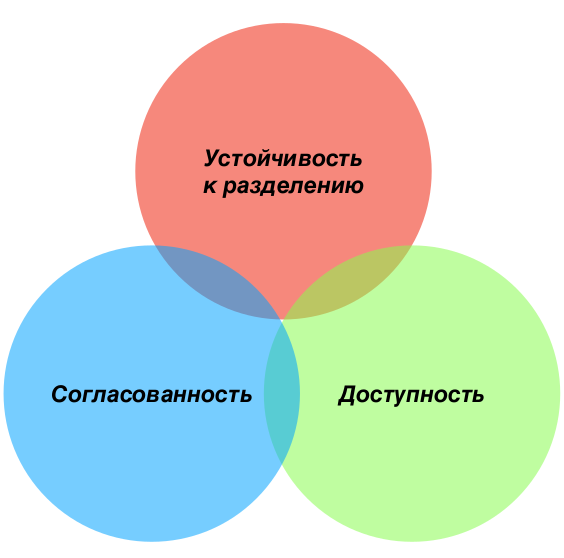
\includegraphics[width=0.5\textwidth]{src/pics/CAP_t.png}
%\caption{CAP теорема}
%\label{ris:image}
%\end{wrapfigure}

CAP-теорема была сформулирована Эриком Брюэром в 2000 году, а через два года доказана. CAP-теорема утверждает, что невозможно создать распределенную систему, которая будет одновременно удовлетворять
% свойству согласованности (то есть её операции записи атомарны, все последующие операции чтения видят новое значение), свойству доступности (система работает, пока работает хотя бы один участник) и свойству устойчивости к потери связности (система продолжает работу, даже если связи между серверами временно отсутствуют), одновременно можно гарантировать только два из этих трех свойств \cite{CAP_Theorem}. 
трём следующим свойствам:
\begin{itemize}
\item \textbf{Согласованности} (consistency) - во всех узлах в один момент времени данные не противоречат друг другу
\item \textbf{Доступности} (availability) - любой запрос к распределённой системе завершается откликом, однако без гарантии, что ответы всех узлов системы совпадают
\item \textbf{Устойчивости к разделению} (partition tolerance) - расщепление распределённой системы на несколько изолированных секций не приводит к некорректности отклика от каждой из секций
\end{itemize}

\begin{figure}[H]
\label{fig:cap_t}
\centering
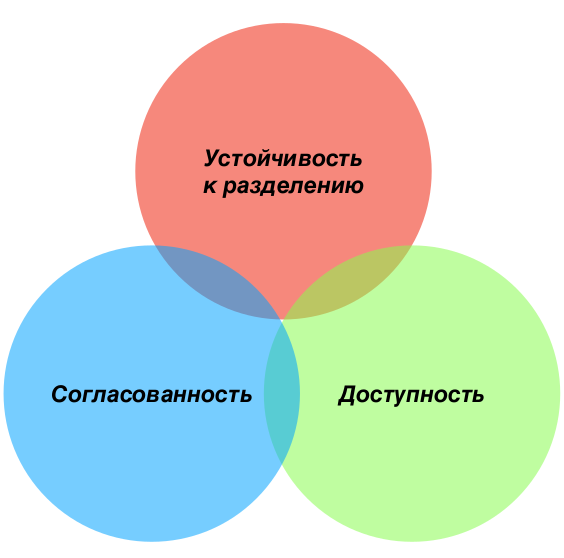
\includegraphics[width=0.6\textwidth]{src/pics/CAP_t.png}
\caption{CAP теорема.}
\end{figure}


Если два узла получают два противоречивых запроса от клиентов, они оба должны принять и обработать запросы, таким образом, ставя под угрозу свойство согласованности или, по крайней мере один из них не должен принимать запрос, таким образом, ставя под угрозу свойство доступности. Как будет видно далее, алгоритм Raft полностью подчиняется этой теореме, он не всегда может быть доступен, но всегда гарантирует согласованность и устойчив к разделению.

\subsection{Распределенный конечный автомат}

Простейший способ реализовать распределённую систему - создать набор клиентов, которые посылают команды избранному центральному узлу-серверу. Сервер должен быть описан как детерминированный конечный автомат, который выполняет в определенном порядке команды от клиентов. Конечный автомат имеет собственное текущее состояние; шаг работы автомата состоит в обработке очередной команды, в результате автомат возвращает ответ клиенту и меняет своё текущее состояние.

Реализация, использующая избранный центральный сервер, не является отказоустойчивой, так как в случае отказа центрального сервера, система перестанет обрабатывать команды клиентов. Таким образом, для
того, чтобы обеспечить отказоустойчивость, системе следует использовать набор серверов, каждый из которых представляет собой детерминированный конечный автомат, то есть все серверы будут выполнять одинаковые последовательности переходов состояний при условии одинаковых входных данных. Клиент, для которого выполняется команда, может использовать любой сервер.

Алгоритмы принятия консенсуса, как правило, возникают в контексте применения распределенных конечных автоматов. При таком подходе, конечные автоматы, расположенные на узлах системы выполняют идентичную команду, находясь в одном и том же состоянии - таким образом, система может продолжать работу, даже если некоторые из его серверов отказывают. Таким образом, распределенные автоматы используются для решения разнообразных проблем отказоустойчивости в распределенных системах.

Распределенные автоматы, как правило, реализуется с помощью реплицированного журнала, как показано на \figref{fig:state_machine}. На каждом сервере хранится реплицируемый журнал, содержащий последовательность команд, которые его собственный конечный автомат выполняет в фиксированном порядке. Каждый журнал содержит одинаковые команды, в одном и том же порядке, так что каждый реплицированный конечный аппарат обрабатывает идентичную последовательность команд. Поскольку конечные автоматы являются детерминированными, каждый обрабатывает идентичную команду при идентичном состоянии и получает идентичные результаты работы.

\vspace{-0cm}
\begin{figure}[H]
\centering
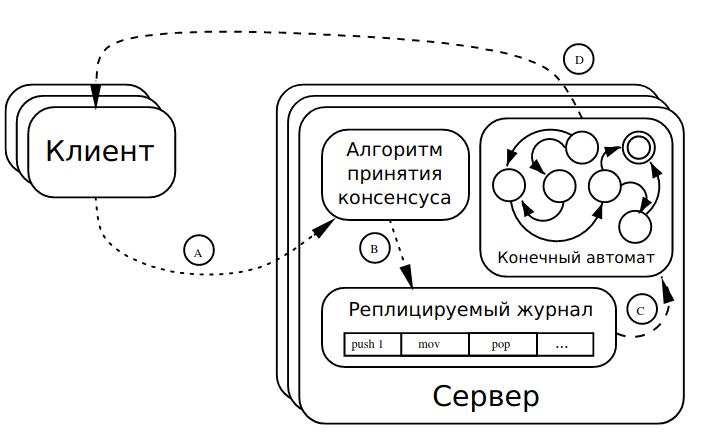
\includegraphics[width=0.82\textwidth]{src/pics/state_machine.png}
\caption{Архитектура системы с использованием распределенного конечного автомата. Алгоритм принятия консенсуса управляет реплицированным журналом, который содержит команды для конечного автомата, которые пришли от клиентов. Конечные автоматы с идентичным состоянием выполняют идентичную последовательность команд из реплицированного журнала, поэтому они порождают одинаковые выходные данные.}
\label{fig:state_machine}
\end{figure}

Поддержание реплицированного журнала согласованным является непосредственной задачей алгоритма принятия консенсуса. Модуль алгоритма принятия консенсуса на сервере получает команды от клиентов
(A) и добавляет их в свой журнал (B). Он общается с модулями алгоритма принятия консенсуса на других серверах, чтобы гарантировать, что каждый журнал в конечном итоге содержит одни и те же команды в
одинаковом порядке, даже если некоторые серверы отказали. После того, как команда клиента успешно реплицируется, конечный автомат каждого сервера обрабатывает их согласно журналу (C), результаты работы возвращаются клиентам (D). В результате система серверов выглядит для клиента как единый, высоконадежный и распределенный конечный автомат.

\subsection{Реализация распределённой системы}

Заключительная задача этой работы, реализация на языке C++ программы, демонстрирующей возможность перестроения централизованной системы в распределённую сеть на основе одного из алгоритмов консенсуса, а также дальнейшее тестирование и сравнение скорости работы получившейся системы. Для чего необходимо провести исследование существующих алгоритмов, детально разобраться в наиболее подходящем из них, после чего использовать его как основу выстраиваемой распределённой системы.

Система хранения, которую необходимо улучшить, является сервером, обрабатывающим клиентские запросы, содержащие в себе данные. В данной системе клиентские запросы производят только запись информации на сервер, дальнейший сбор которых происходит отдельными средствами на самом сервере. При получении запроса сервер записывает обратившегося и считает, что этот клиент занял некоторое абстрактное мест, которое в дальнейшем будем называть \emph{слот}. Если клиент долгое время не посылал запросов, сервер считает, что "слот"\ освобожден. Таких "слотов"\ на сервере ограниченное количество.
Клиентский запрос должен содержать набор данных фиксированного размера, который состоит из двух частей: уникальная часть, в качестве информацию о себе, и информация, необходимая для сохранения на сервере. Ответ сервера содержит лишь информацию о том, удалось принять запись или нет.

\newpage
\section{Основная часть}

\subsection{Различные алгоритмы консенсуса}

Рассмотрим свойства распределённой системы, перечисленные в CAP теореме. Одно из этих свойств не будет удовлетворенно в распределённой системе, которую мы хотим построить. 

Если отказаться от устойчивости к разделению, то такая система потеряет одно из своих основных преимуществ, а именно отказоустойчивость, так как при отделении даже одного узла, система не сможет корректно обработать ни один запрос.

Свойство согласованности игнорировать полностью также нельзя, так как в таком случае распределённая система может разделиться на несколько самостоятельных частей, никак не согласовывающих ответы на запросы. 

Если же рассматривать оставшиеся варианты, можно разделить алгоритмы следующим образом:

\begin{figure}[H]
\centering
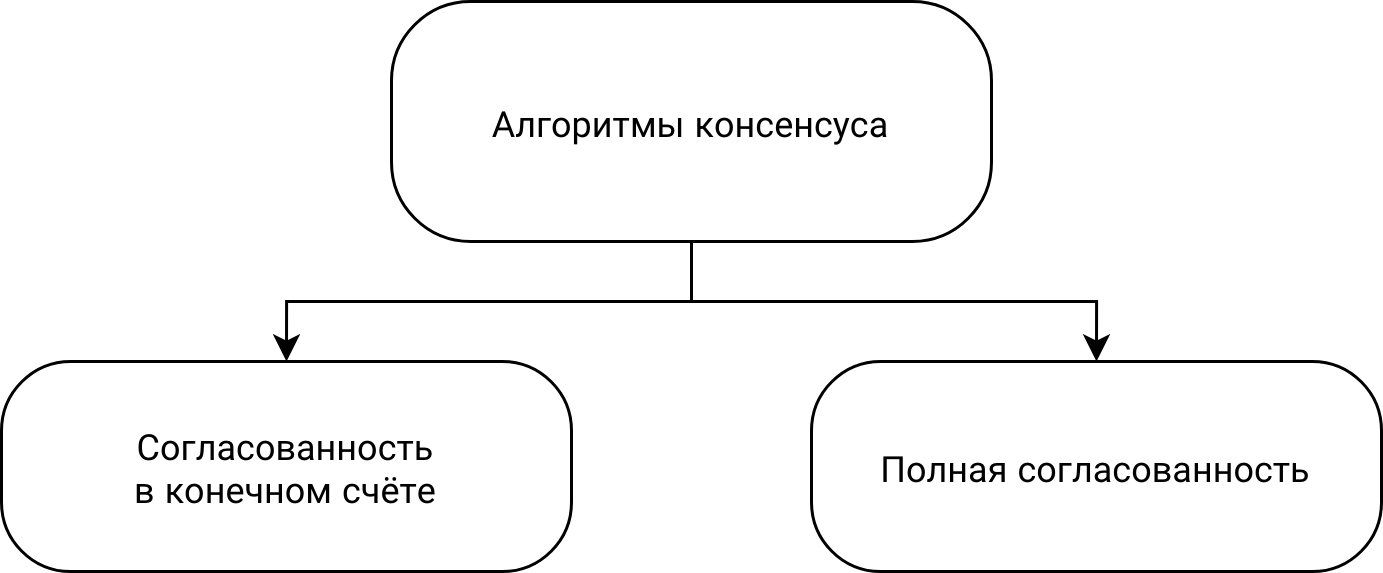
\includegraphics[width=1\textwidth]{src/pics/consensus_types_1.png}
\caption{Разделение алгоритмов по типу согласованности.}
\label{fig:consensus_types_1}
\end{figure}

\emph{Полная согласованность} - это в точности то, что определяется в CAP теореме.

\emph{Согласованность в конечном итоге} - это свойство, при котором гарантируется, что в отсутствии изменений данных, через какой-то промежуток времени после последнего обновления ("в конечном счёте") все запросы будут возвращать последнее обновлённое значение.

Согласованность в конечном итоге позволяет удовлетворить свойство доступности и соответственно используется в системах, её требующих.

В качестве примеров, выше описанного разделения, рассмотрим следующие алгоритмы консенсуса:

\subsubsection{Алгоритмы с согласованностью в конечном итоге}

\begin{figure}[H]
\centering
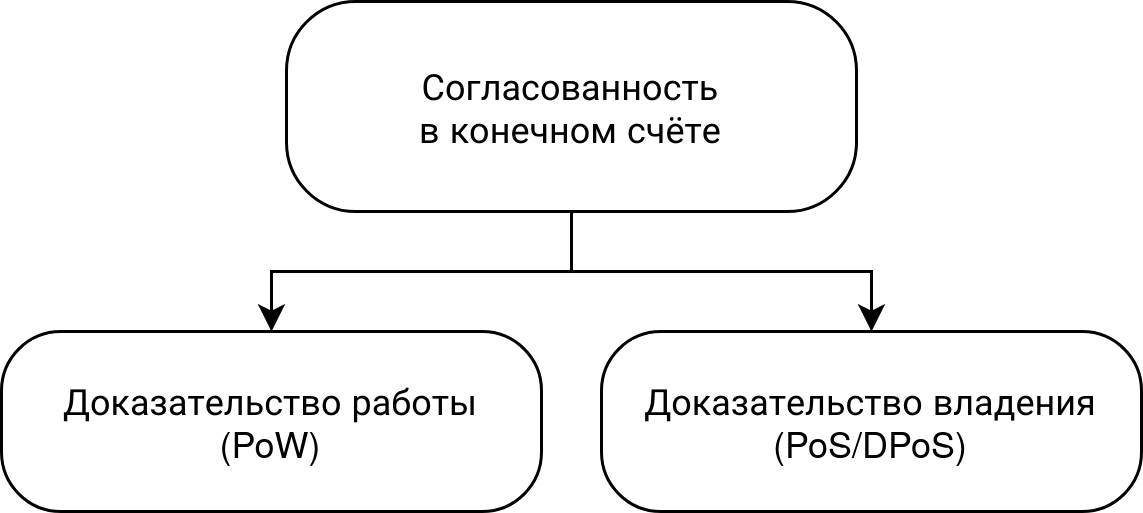
\includegraphics[width=0.8\textwidth]{src/pics/consensus_types_2.png}
\caption{Примеры алгоритмов, согласованных в конечном итоге.}
\label{fig:consensus_types_2}
\end{figure}


\subsubsection{"Доказательство работы"\ (PoW)}

"Доказательство работы"\ - ("Proof-of-Work") - один алгоритмов консенсуса, использующиеся в системах с высокой доступностью. PoW выбирает один узел для создания новой записи в каждом раунде консенсуса с помощью конкуренции узлов в вычислении некоторого хэша. Узел, который первым решит эту "криптографическую головоломку"\, имеет право на создание записи и присоединение её к самой длинной цепочке из существующих, которая считается правильной. Соответственно, для увеличения шансов получения новой записи требуется большая вычислительная мощность. 

Для поддержания работы такой системы, каждый узел должен совершать множество вычислений, поэтому, для поддержания заинтересованности в этом узлов, успешные вычисления вознаграждаются записью об этом внутри самой системы.

Потенциально существует ненулевая вероятность, что злоумышленник может переписать запись или иметь скрытую более длинную цепочку, и тогда именно его версия цепочки будет верной, что является угрозой для остальных пользователей. Однако с ростом числа пользователей такая вероятность стремится к нулю, так как требует огромных вычислительных затрат: больше половины всех вычислительных мощностей (что известно как "атака 51"). Таким образом, в PoW транзакция может быть отменена, но с течением времени эта возможность значительно усложняется. Следовательно, PoW выбирает доступность и устойчивость к разделению; согласованность обеспечивается лишь в конечном счете. Использование PoW ведет к огромным тратам вычислительных ресурсов и по сути бессмысленным вычислениям хэш-функций, вычисленные результаты которых нигде более не используются.

\subsubsection{"Доказательство доли владения"\ (PoS)}

"Доказательство доли владения"\ - (Proof-of-Stake) -  этот алгоритм был разработан для решения проблемы большой вычислительной сложности алгоритма PoW,  алгоритм обеспечивает большие шансы на право создания новой записи тем, кто имеет большую долю имеющегося вознаграждения, выданного данной системой ранее, от общего её количества (в отличие от большей доли вычислительных мощностей в PoW). В PoS также применяется решение "криптографической головоломки"{} , однако её вычисление менее затратно и зависит от внесённого ранее вклада этого узла, по созданию предыдущих записей. Это позволяет экономить значительные вычислительные ресурсы, однако такая схема ведёт к увеличению влияния на систему наиболее активных узлов, что сказывается на всё большей централизации сети. Кроме того, существует вероятность "сговора"\ узлов, что даёт им возможность навязывать свои условия вне зависимости от мнения большого числа узлов.

\subsubsection{"Делегированное доказательство доли владения"\ (DPoS)}
"Делегированное доказательство доли владения"\ - (Delegated Proof-of-Stake) - позволяет узлам, имеющих долю вознаграждения, голосовать за выбор создателей (верификаторов) записей, то есть делегировать право создания записей другим узлам, тем самым снижая собственные вычислительные затраты до нуля. Вес голоса участника при делегировании пропорционален той доле, что он имеет. Делегаты получают некоторое вознаграждение за каждую созданную запись.  В случае неудачи в создании записи за определенное время выбирается следующий узел.

Таким образом, DPoS заметно менее вычислительно затратный по сравнению с PoW и PoS. Также этот алгоритм предлагает больше влияния узлам, которые имеют не такую большую долю, как другие узлы. В PoS и DPoS действующая на данный момент цепочка записей может быть изменена, хоть реализация этого достаточно сложна, и алгоритм является согласованным в конечном итоге. Тем не менее, сеть останется доступной и продолжит работу, даже если она позволяет проводить неточные транзакции.

\subsubsection{Алгоритмы с полной согласованностью}

В алгоритмах с полной согласованностью для обеспечения устойчивости к разделению, требуется дублирование изменений во всех узлах программной системы. Которое часто обеспечивается алгоритмами голосования \cite{Blockvhain_review}.
Алгоритмы консенсуса, базирующиеся на голосованиях, делятся на две категории: BFT (Byzantine Fault Tolerance — отказоустойчивость к византийским ошибкам) и CFT (Crash Fault Tolerance — отказоустойчивость к падениям узлов). Если алгоритмы второй категории не чувствительны к падениям узлов по чисто техническим причинам, то первые также работают и при "византийском"\ поведении некоторых участников, когда те ведут себя злонамеренно и пытаются ввести в заблуждение другие узлы.

\begin{figure}[H]
\centering
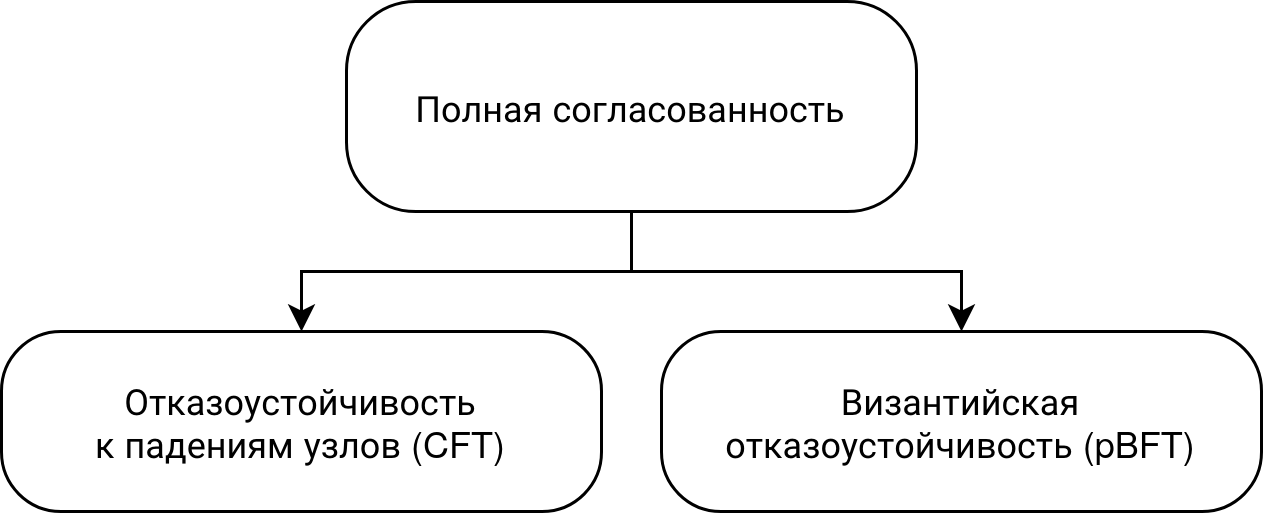
\includegraphics[width=0.85\textwidth]{src/pics/consensus_types_3.png}
\caption{Деление алгоритмов с полной согласованностью.}
\label{fig:consensus_types_3}
\end{figure}

\subsubsection{Практическая византийская отказоустойчивость}

Одной из простейших реализаций BFT является алгоритм "Практическая византийская отказоустойчивость"\ (Practical Byzantine Fault Tolerance) \cite{Byzantine_Fault_Tolerance}. Данный алгоритм обладает низкой вычислительной сложностью и высокой практичностью в распределенных системах. В данном протоколе узлы выбирают узел-лидер в рамках циклического механизма. Лидер является таковым до тех пор, пока сам не выйдет из строя, после чего выбирается новый лидерский узел. Корректная работа алгоритма лежит в предположении, что все корректно работающие узлы имеет одинаковый набор записей. Число злонамеренных и выведенных из строя узлов должно быть строго меньше $1/3$ от общего количества участников. Таким образом, чем больше узлов в сети, тем менее вероятно, что треть или более узлов будут мошенническими или выведенными из строя. 

Процесс генерации записи в pBFT консенсусе может быть описан следующим образом. Клиент отправляет запрос узлу, который был выбран лидером, для создания записи. Лидер собирает запросы на создание записей и группирует их в блок. Затем блок рассылается всем остальным узлам в сети. Каждый узел верифицирует записи в блоке, создает другой блок с действительными записями, вычисляет хэш-функцию от этого блока и рассылает это другим узлам. Узел ожидает ответа от $2/3$ узлов с тем же хэшем, после чего блок добавляется последовательности записей этого узла.

Такой механизм обеспечивает поддержание одинакового для всех узлов набора записей и строгой согласованности, то есть однажды добавленная запись уже не может быть недействительной. Выбор лидерского узла обозначает некоторый уход от полной децентрализации, но такой подход является отличным решением для приватных сетей, так как большое число пересылок сообщений показывает pBFT как алгоритм, эффективный в системах с малой задержкой, но чувствительный к числу участников

\subsubsection{Raft}

Примером Crash Fault Tolerance (CFT) алгоритма может служить протокол Raft (расшифровка отсутствует) \cite{Raft_search}. Проблема издержек связи в виде большого числа пересылок при pBFT устраняется в алгоритме Raft в предположении, что коммуникация в сети происходит только через лидерский узел. Как и любой CFT алгоритм, Raft обеспечивает безопасность только в ситуациях возможных сбоев узлов без защиты от злонамеренных атак. Правильная работа механизма обеспечивается при более чем половины рабочих узлов. Все узлы могут быть в одной из следующих ролей: лидер (только один), кандидат в лидеры (в случае отсутствия такового) или ведомый. Именно лидер отвечает за создание записей при получении запросов от клиентов. Весь процесс работы сети может быть представлен как три этапа: избрание лидера, репликация набора записей и выполнение записей.

Raft консенсус не работает со злонамеренным поведением узлов. Если такое поведение наблюдается у лидера или у большинства узлов, то набор записей становится недействительным. Так как только один узел может дополнять набор (но не изменять предыдущие записи), то Raft не подвержен проблеме дублирования записей. Raft предпочтителен для небольших сетей, так как с ростом числа участников значительно растет число сообщений, что определяет данный консенсус как применимый в приватных сетях. Для нормальной работы сети требуется, чтобы время доставки сообщений от узлов к лидеру и наоборот было намного меньше времени голосования, которое в свою очередь должно быть намного меньше времени стабильной работы узлов в сети (то есть времени работы без отказов). Данный алгоритм консенсуса обладает свойством строгой согласованности.

%\newpage
\subsubsection{Сравнение алгоритмов}

Как итог сравнения перечисленных алгоритмов можно составить таблицу таких характеристик, как:
\begin{itemize}
\item Согласованность - полная или в конечном счёте
\item Отказоустойчивость - количество единичных отказов узлов системы из $N$ узлов, после наступления которых сохраняется работоспособность системы в целом. 
\item Вычислительная сложность - оценка количества вычислений, требующихся для принятия консенсуса.
\item Масштабируемость - способность системы справляться с увеличением нагрузки с увеличением количества узлов.
\end{itemize}

\begin{table}[H]
\begin{center}
\begin{tabular}{|c|c|c|c|c|}
\hline
Свойство & PoW & PoS/DPoS & pBFT & Raft \\
\hline
Согласованность & \multicolumn{2}{c}{В конечном счёте} & \multicolumn{2}{|c|}{Полная}    \\
\hline
Отказоустойчивость & \multicolumn{2}{c|}{$N/2$} & $N/3$ & $N/2$  \\
\hline
Вычислительная сложность  & Высокая & Низкая & \multicolumn{2}{c|}{Незначительная}  \\
\hline
Масштабируемость & \multicolumn{2}{c|}{Высокая} & \multicolumn{2}{c|}{Низкая}  \\
\hline
\end{tabular}
\end{center}
\caption{Сравнение алгоритмов консенсуса.  $N$ (для параметра отказоустойчивости) - общее количество узлов в системе.}
\end{table} 

В результате изучения алгоритмов, для детального изучения и реализации был выбран алгоритм Raft. Так как для распределённой реализации имеющегося сервера важна полная согласованность, нет возможности возникновения византийской проблемы и нет необходимости создания большой сети узлов. Также этот алгоритм является достаточно новым (2014 год), и интересен с точки зрения реализации и тестирования. 

\subsection{Подробное описание алгоритма Raft}

Алгоритм Raft - это алгоритм консенсуса, разработанный для обеспечения надежности и отказоустойчивости в распределенных системах. Он основан на идее выбора лидера среди узлов системы, который затем координирует работу всех остальных узлов. Raft разбивает процесс выбора лидера и репликации данных на два независимых шага, что облегчает понимание и реализацию алгоритма. При помощи голосования и случайных таймаутов Raft выбирает лидера, который затем управляет репликацией данных и поддержанием консистентности. Алгоритм Raft обеспечивает высокую устойчивость к отказам узлов и позволяет системе продолжать работу при сбоях и разрывах связи.
Данные, обслуживаемые системой с Raft, представляют собой лог, состоящий из записей. Когда пользователь хочет изменить данные, хранящиеся в системе, он добавляет в лог новую запись с командой.

\subsubsection{Основные понятия}

Каждый узел может находится в одном из 3-х состояний:
\begin{enumerate}[noitemsep,topsep=-5pt,parsep=-5pt,partopsep=-5pt]
\item Лидер - обрабатывает все клиентские запросы, поддерживает актуальность лога.
\item Кандидат - специальное состояние сервера, возможное только во время выбора нового лидера.
\item Ведомый - сервер, который только добавляет записи в лог от лидера и перенаправляет все входящие запросы от клиентов на лидера.\
\end{enumerate}
\
Возможные переходы между состояниями описаны следующим рисунком:
%\vspace{-0.7cm}
\begin{figure}[H]
\centering
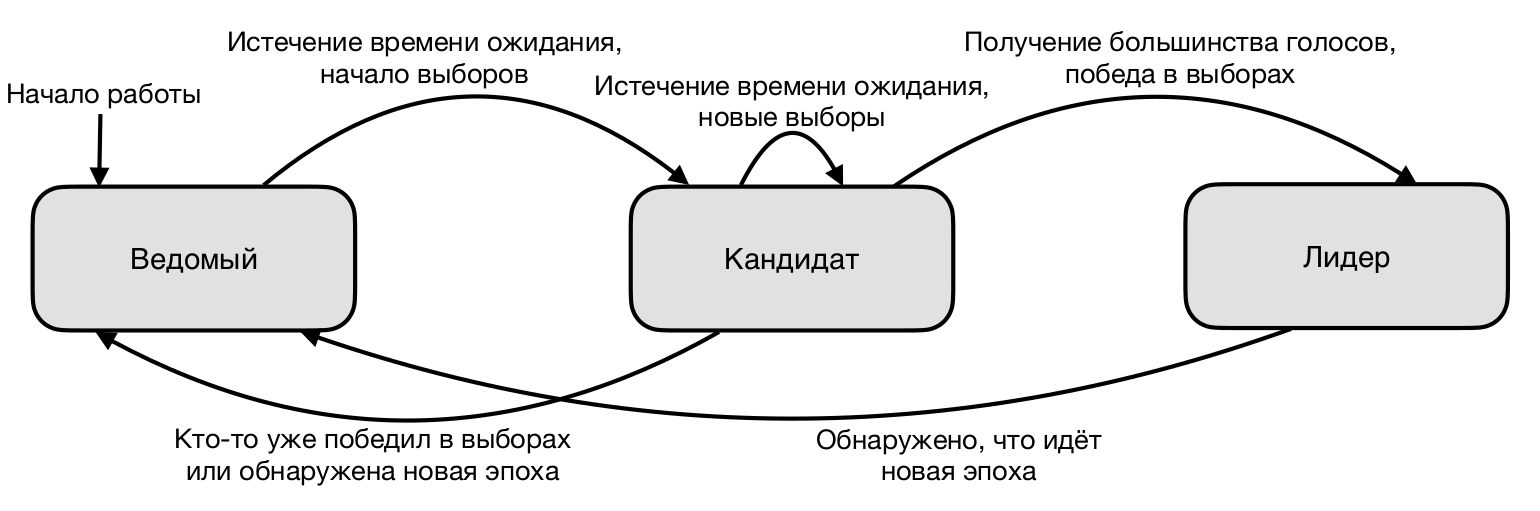
\includegraphics[width=1\textwidth]{src/pics/states.png}
\caption{Возможные статусы сервера и переходы между ними. Если ведомый не получает контрольных сообщений, он становится кандидатом и инициирует выборы. Кандидат, получивший голоса большинства участников всей сети, становится новым лидером.}
\label{fig:states}
\end{figure}

Во время нормальной работы в системе только один сервер является лидером, все остальные – его ведомые.

Управление системой четко разделено на две фазы:
\begin{enumerate}
\item Выборы лидера (голосование)
\item Репликация (передача данных протокола)
\end{enumerate}

Raft делит время на отрезки произвольной длины, называемые эпохами. Каждая эпоха имеет монотонно возрастающий номер. Эпоха начинается с выборов лидера, когда один или несколько серверов становятся кандидатами. В случае, если кандидат получает большинство голосов, он становится лидером до конца данной эпохи. Если же голоса разделились, и ни один из кандидатов не может получить большинство голосов, срабатывает таймаут, и эта эпоха заканчивается. После этого начинается новая с новыми кандидатами и выборами. Пример проиллюстрирован эпохой номер три на следующей диаграмме:

\begin{figure}[H]
\centering
\vspace{0.4cm}
\hspace*{0.2cm}
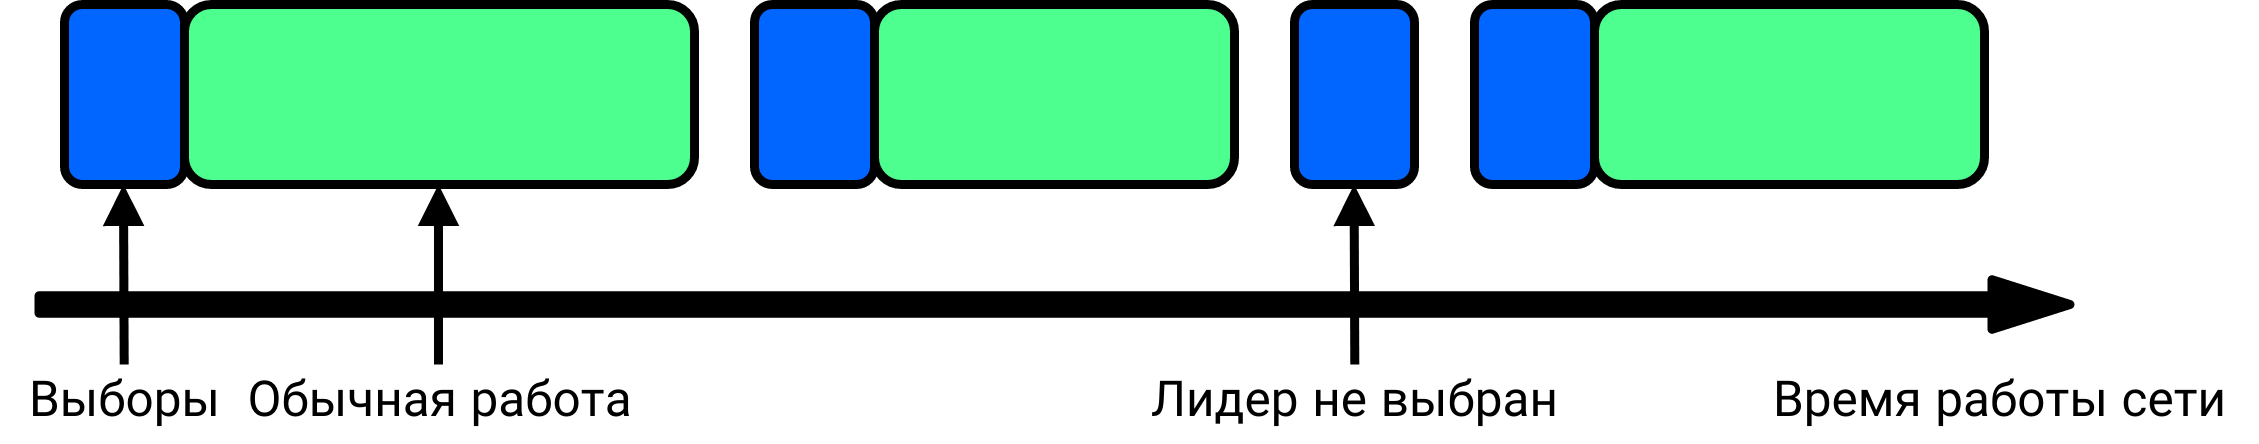
\includegraphics[width=1\textwidth]{src/pics/terms.png}
\caption{Время делится на эпохи, и каждая эпоха начинается с процедуры выборов лидера. После успешных выборов, лидер управляет системой до конца эпохи. Некоторые выборы заканчиваются неудачно, и в этом случае эпоха заканчивается без выбора лидера. Переходы между эпохами можно наблюдать в различные моменты времени на различных серверах.}
\label{fig:terms}
\end{figure}

Raft гарантирует, что существует не более одного лидера в отдельно взятой эпохе.
Номер эпохи помогает серверам в системе Raft определять, какая информация более актуальна на текущий момент. 
Различные сервера могут наблюдать переходы между эпохами в различное время, а в некоторых ситуациях сервер может по какой-либо видеть не наблюдать отдельные выборы или даже целые эпохи. Эпохи действуют в качестве логических часов в Raft; они позволяют обнаруживать сервера с устаревшей информацией, например такой, как "устаревшее"\ лидерство.

Правила взаимодействия серверов и эпох
\begin{itemize}
\item Каждый сервер отслеживает номер своей текущей эпохи.
\item Сервер включает номер своей эпохи в каждое отправляемое сообщение.
\item Если сервер получает сообщение с меньшим номером эпохи, чем его собственный, то он игнорирует это сообщение.
\item Если ведомый сервер получает сообщение с большим номером эпохи, чем его собственный, то он обновляет свой номер эпохи, чтобы тот соответствовал полученной.
\item Если кандидат или лидер получает сообщение с большим номером эпохи, чем его собственный, то он понимает, что другие сервера уже инициировали новую эпоху, а его более неактуальна. Поэтому он переходит из текущего состояния в состояние ведомого вдобавок к обновлению своего номера.
\end{itemize}


Серверы в Raft взаимодействуют посредством обмена запросами и ответами. Базовый алгоритм использует всего два вида вызовов: 
\begin{itemize}
\item \emph{RequestVote} используется кандидатами во время выборов. Запрос содержит номер эпохи кандидата и метаданные о логе кандидата, более подробно рассмотренные далее. Ответ содержит номер эпохи отвечающего сервера и значение «true», если сервер голосует за кандидата; «false», если сервер голосует против кандидата.
\item \emph{AppendEntries} используется лидером для репликации лога, а также для механизма heartbeat. Запрос содержит номер эпохи лидера, коллекцию записей, которые нужно добавить в лог (или пустую коллекцию в случае heartbeat), некоторые метаданные о логе лидера, также подробнее рассмотренные далее. Ответ содержит номер эпохи ведомого и значение «true», если ведомый успешно добавил записи в свой лог; «false», если добавить записи в лог не удалось.
\end{itemize}

\subsubsection{Алгоритм  работы}

\textbf{1. Процедура выборов.}\\
Raft использует механизм периодических контрольных сообщений для управления состоянием системы, в том числе, для проведения выборов лидера, когда они нужны. При запуске сервера начинают свою работу в состоянии ведомых. Сервер остается в состоянии ведомого до тех пор, пока он получает корректные сообщения от лидера или кандидатов. Лидер периодически отправляет контрольные сообщения путем вызова \emph{AppendEntries} для всех ведомых(в том числе и в ситуации, когда нет новых записей для добавления в журнал нет). Если ведомый не получает сообщения от лидера в течение определенного периода времени под названием "период ожидания выборов", то он предполагает, что лидера
больше нет, и начинает выборы, чтобы избрать нового лидера. 

Для того, чтобы начать выборы, ведомый увеличивает свой номер эпохи и переходит в состояние кандидата. Затем голосует за себя, взводит внутренний таймер и параллельно вызывает \emph{RequestVote} для каждого из других серверов в системе. Кандидат продолжает оставаться в таком состоянии до тех пор, пока не случится одно из этих событий:
\begin{itemize}
\item кандидат побеждает на выборах
\item другой кандидат побеждает и устанавливает себя в качестве лидера
\item ничья; эпоха заканчивается без лидера
\end{itemize}

\textbf{\textit{1.1. Победа в выборах.}}\
Кандидат побеждает на выборах, если он получает в той же эпохе голоса "за"\ от большинства серверов всей системы. Каждый сервер будет голосовать как минимум за одного кандидата в отдельно взятой эпохе, по принципу FIFO (отдаёт свой голос за первого полученного кандидата, например в случае инициации голосования - за себя). Необходимость большинства голосов "за"\ для победы гарантирует, что не более, чем один кандидат может победить на выборах для конкретной эпохи. После того, как кандидат побеждает на выборах, он становится лидером и начинает отправляет периодические контрольных сообщения всем другим серверам, чтобы подтвердить своё лидерство и предотвратить новые выборы.

\textbf{\textit{1.2. Победа другого кандидата.}}
В ожидании голосов, кандидат может получить AppendEntries от другого сервера, который является лидером. Если номер эпохи лидера (которые передается как один из параметров сообщения) не меньше, чем у кандидата, то кандидат признает лидера законным и возвращается в состояние ведомого. Если номер эпохи лидера в сообщении меньше текущей эпохи кандидата, то кандидат отвергает сообщение и продолжается оставаться в состоянии кандидата

\textbf{\textit{1.3. Ничья.}}
Третий возможный исход, состоит в том, что кандидат ни побеждает, ни проигрывает выборы: если много ведомых попытаются стать кандидатами в приблизительно одно и то же время, голоса могут быть разделены таким образом, что ни один кандидат не получит большинство. Когда это происходит, у кандидов начинают истекать внутренние таймера (перед выборами каждый кандидат выставляет свой собственный таймер и запускает его). Затем, каждый кандидат с вышедшим таймером попробует начать новые выборы, увеличивая номер эпохи и начиная новый раунд вызовом RequestVote для всех остальных серверов. Без дополнительных мер "ничья"\ может повторяться до бесконечности. \\


Raft использует рандомизированные таймера, чтобы обеспечить, что ситуации "ничьих"\ будут редки, а если они и случатся, то будут разрешены быстро. Чтобы предотвратить такие ситуации, интервалы срабатывания таймеров для кандидатов и ведомых выбираются случайным образом из фиксированного диапазона (например, 150-300 миллисекунд). Это приводит к тому, что в большинстве случаев только один ведомый начинает выборы; он выигрывает выборы и посылает контрольное сообщение до того, как у любых других серверов сработает таймер. Тот же механизм используется для обработки "ничьих"\ во время выборов. Каждый кандидат перезапускает его рандомизированный таймер в начале выборов, и ждет истечения таймера, чтобы начать новые выборы. \\


Иллюстрация работы сети в момент инициализации (\figref{fig:init}) и отказа лидера в процессе работы (\figref{fig:elec}):

%\vspace{-5.4cm}

\begin{figure}[H]
\begin{minipage}[h]{0.46\linewidth}
\center{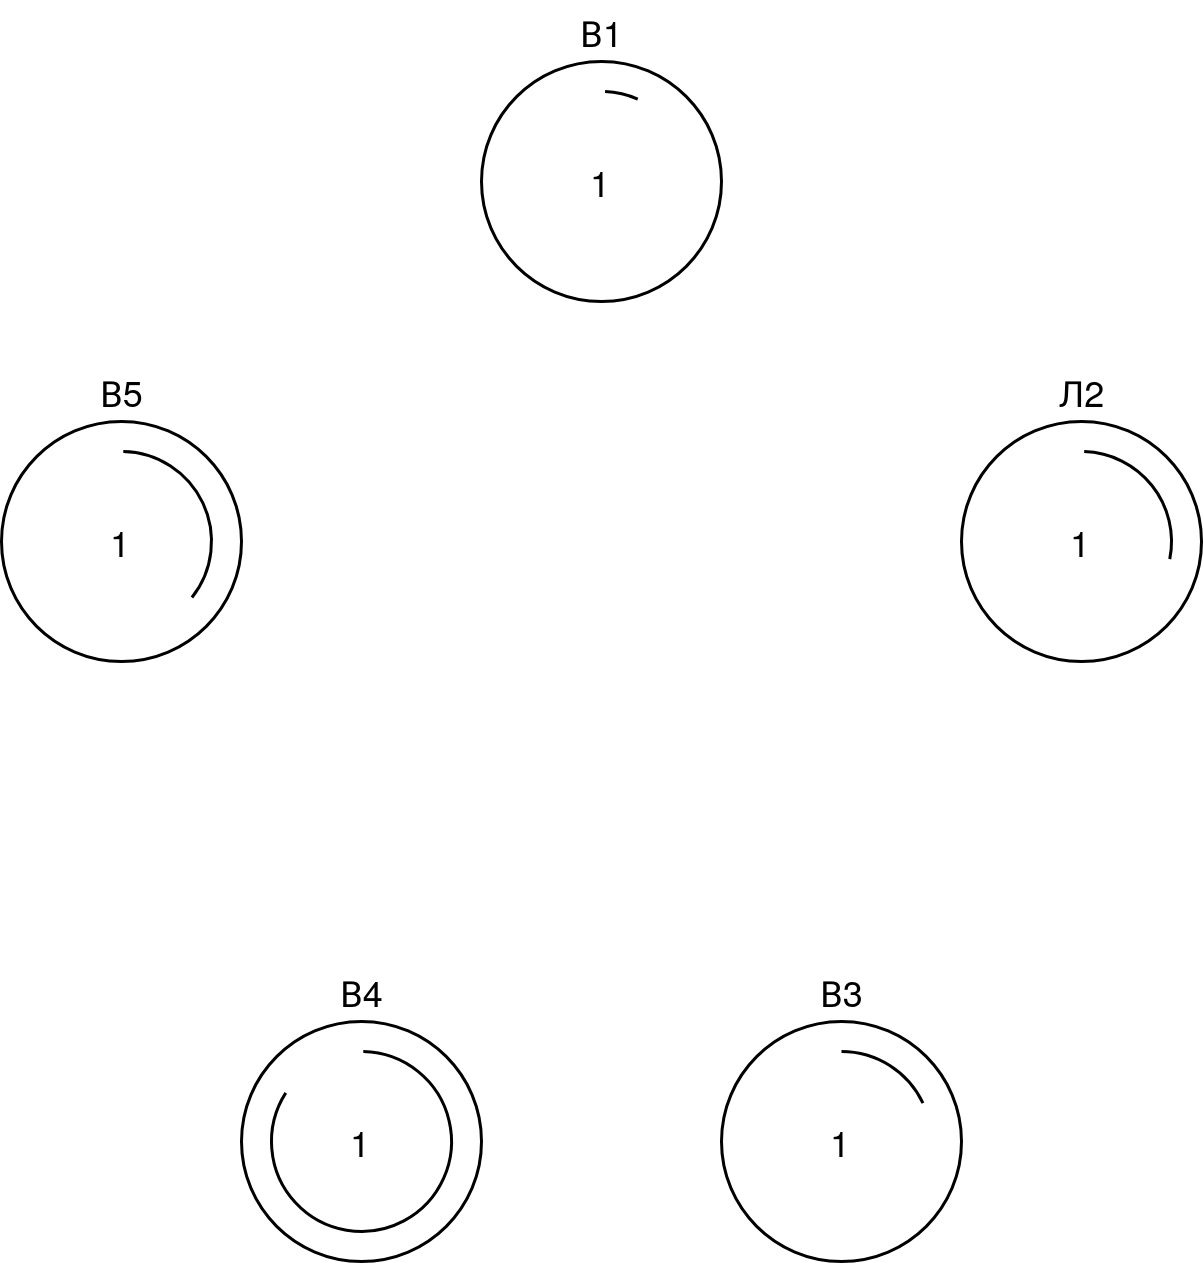
\includegraphics[width=1\linewidth]{src/pics/init_1.png}} 
\begin{small}
Начальное состояние, все сервера являются ведомыми. Так как у В4 рандомизированный таймер сработает раньше других, В4 раньше перейдет в состояние кандидата, начнет выборы. \\
\end{small}
\end{minipage}
\hfill
\begin{minipage}[h]{0.46\linewidth}
\vspace{-0.2cm}
\center{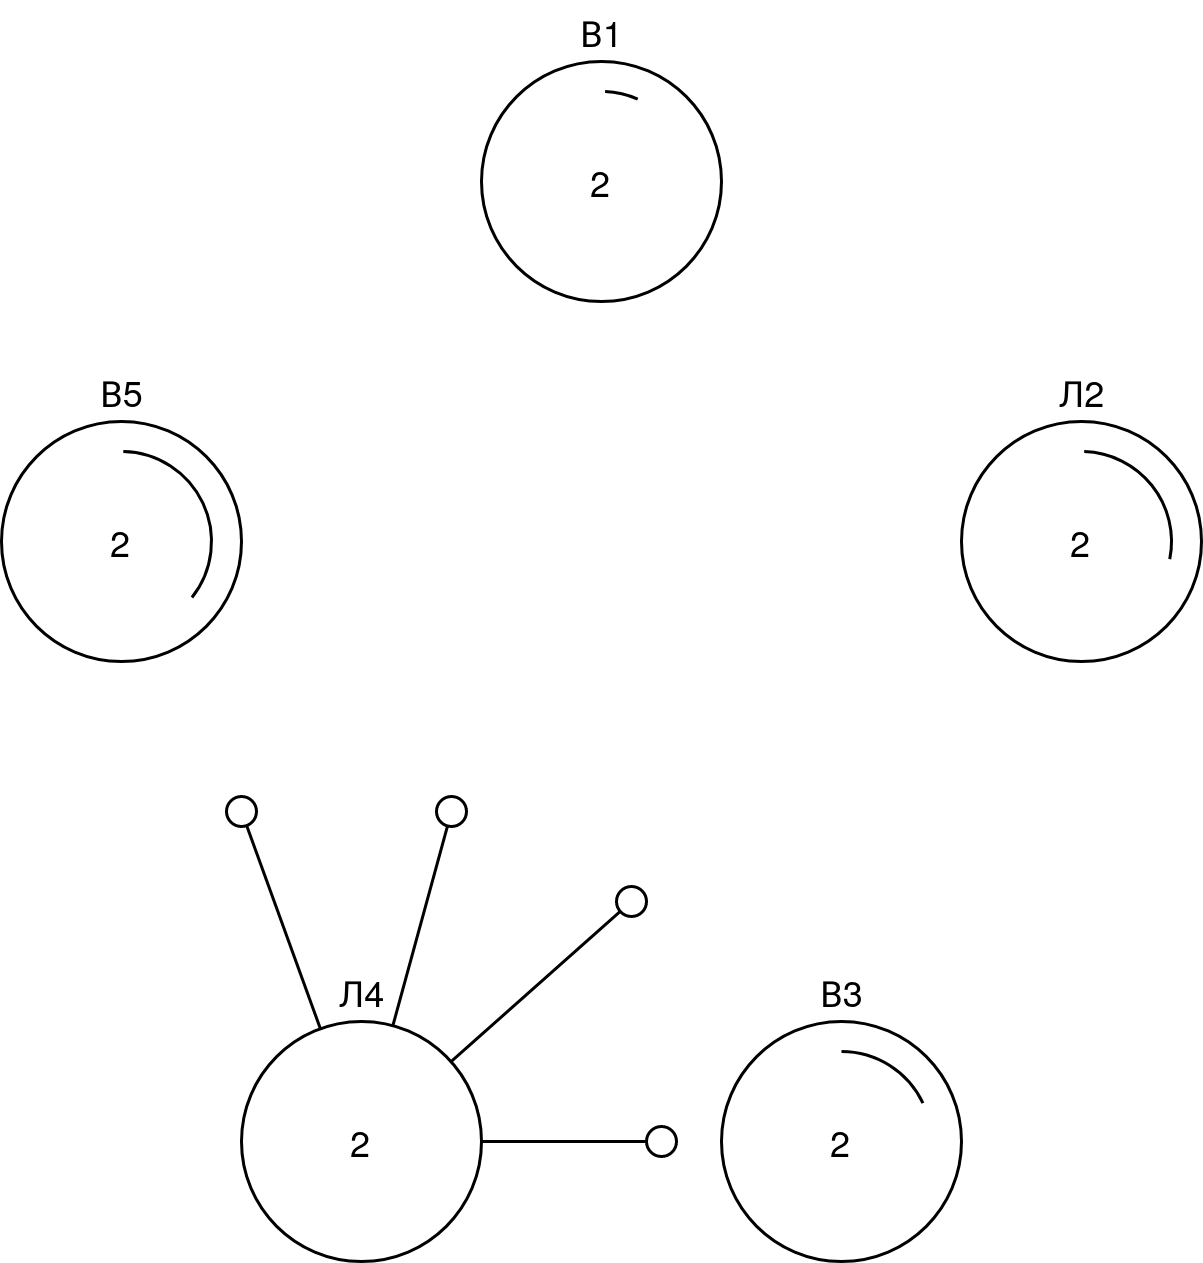
\includegraphics[width=1\linewidth]{src/pics/init_2.png}} \\
\begin{small}
Выборы прошли успешно для узла Л4, он стал лидером и начал периодически отправлять контрольные сообщения всем ведомым.
\end{small}
\end{minipage}
\caption{}
\label{fig:init}
\end{figure}

\
\newpage
\begin{figure}[H]
\vspace{-1cm}
\begin{minipage}[h]{0.46\linewidth}
\center{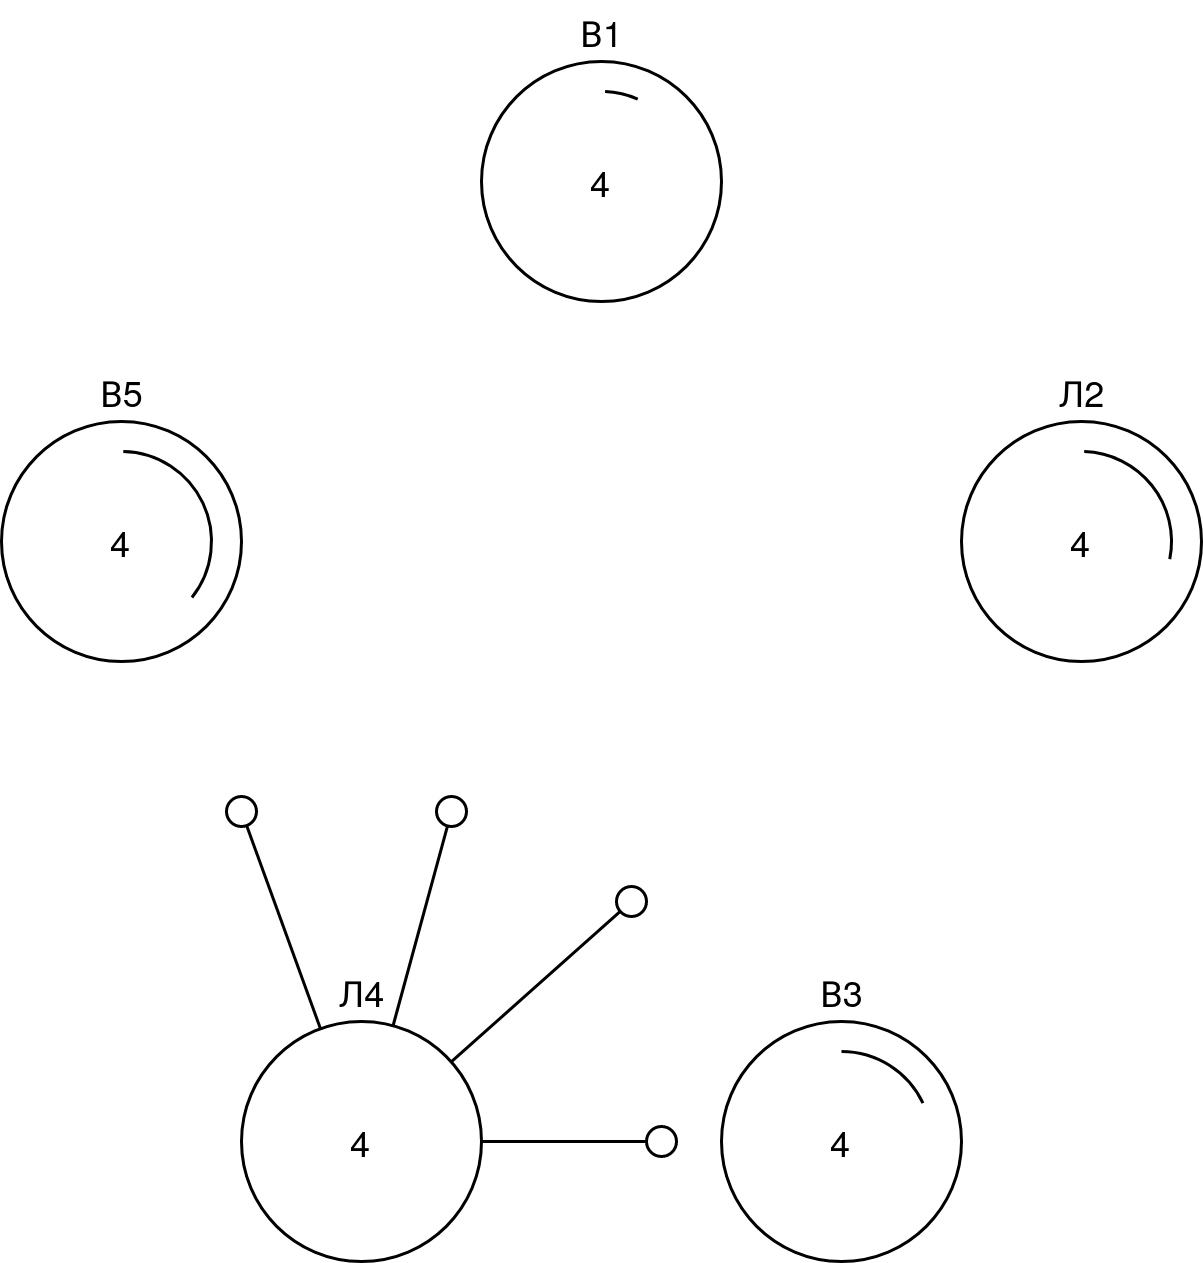
\includegraphics[width=1\linewidth]{src/pics/elec_1.png}} 
\begin{small}
Система находился в эпохе номер 4, с лидером Л4, который рассылает контрольные сообщения ведомым. \\
\end{small}
\end{minipage}
\hfill
\begin{minipage}[h]{0.46\linewidth}
\vspace{0.6cm}
\center{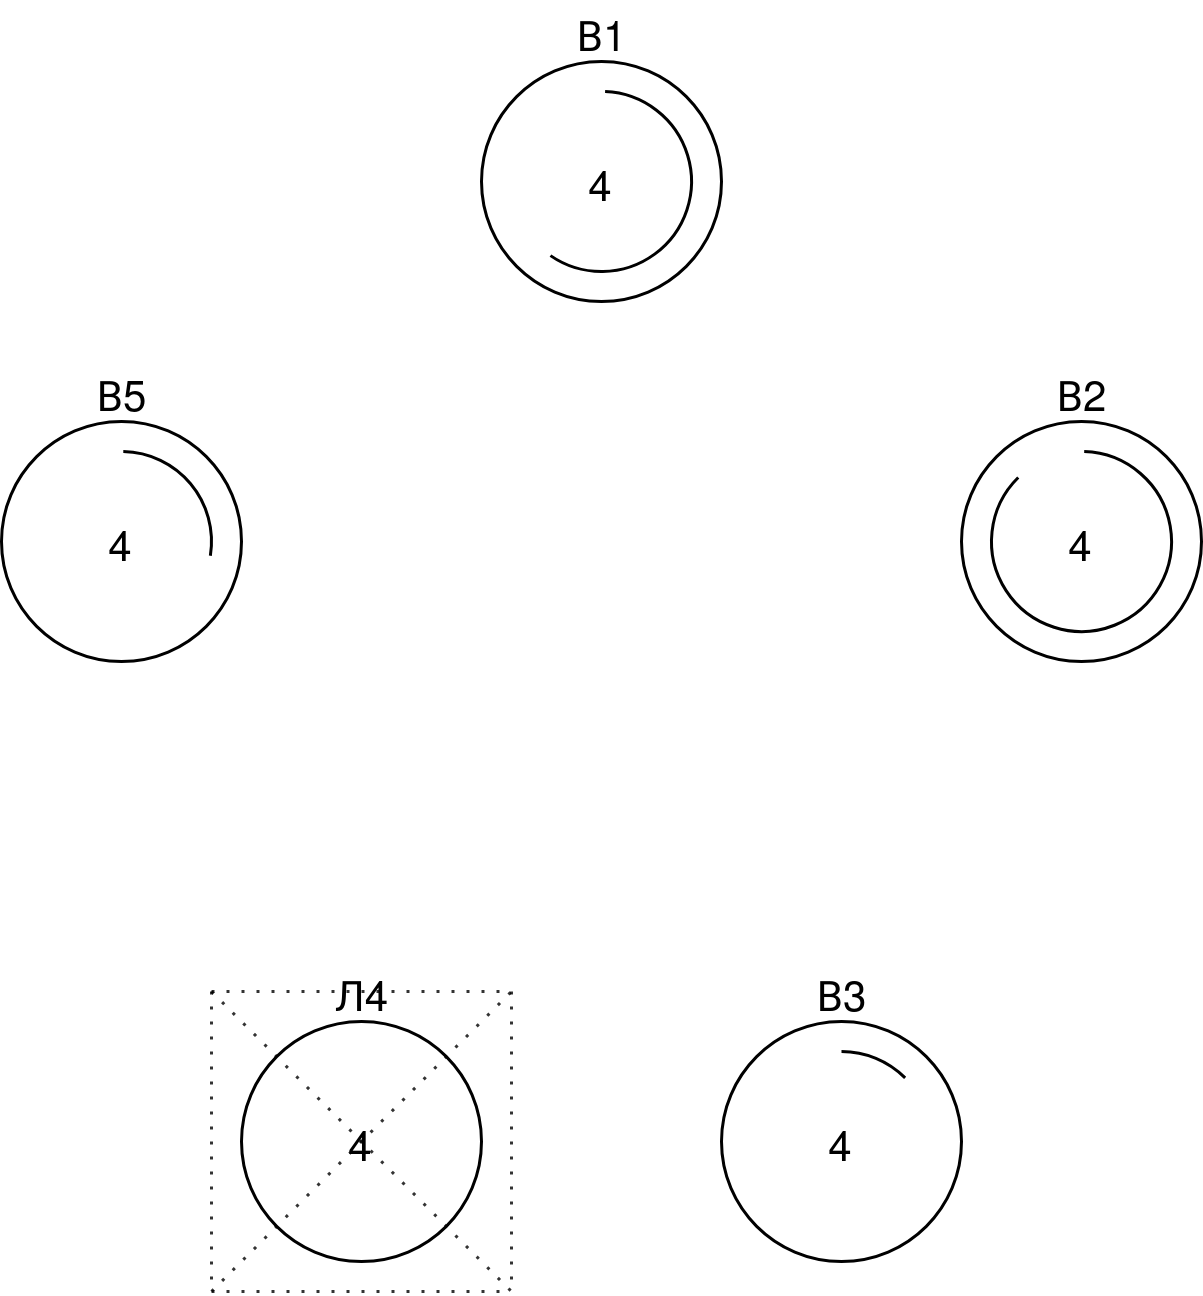
\includegraphics[width=1\linewidth]{src/pics/elec_2.png}} \\
\begin{small}
Лидер Л4 отказывает. Без контрольного сообщения от лидера, таймеры ведомых не обновляются и начнётся голосование.
\end{small}
\end{minipage}
\vfill
\begin{minipage}[h]{0.46\linewidth}
\center{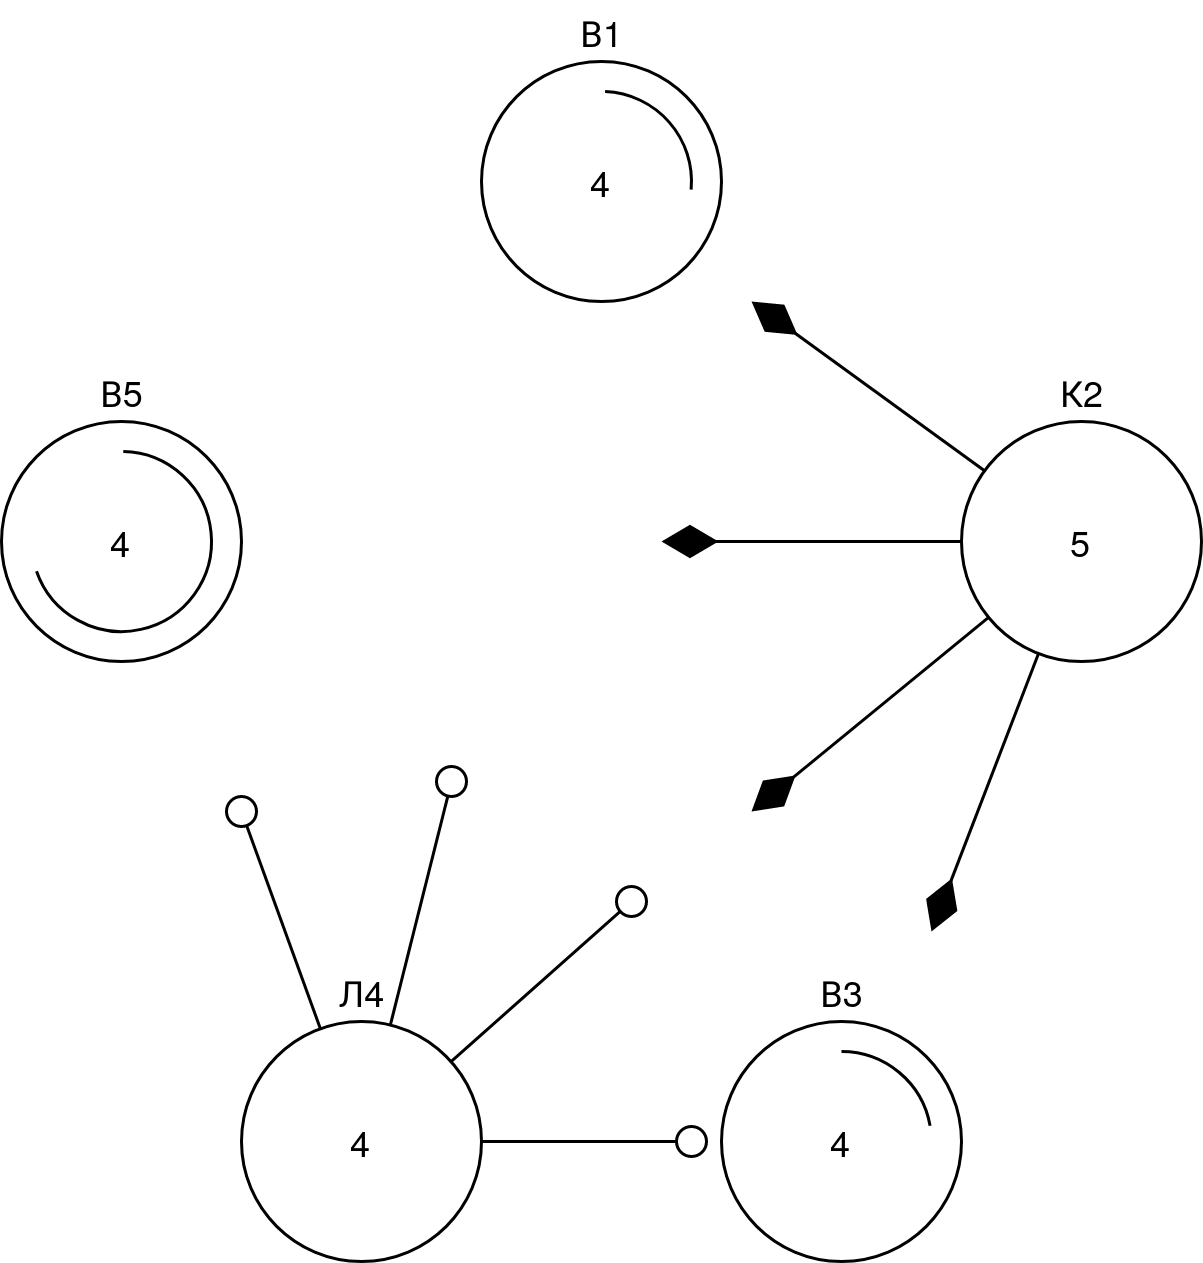
\includegraphics[width=1\linewidth]{src/pics/elec_3.png}} 
\begin{small}
Сервер К2 становится кандидатом, увеличивает номер своей эпохи, и отправляет всем серверам сообщение с началом голосования. В это же время сервер Л4 восстанавливается после сбоя, и посылает контрольное сообщение всем серверам для подтверждения своего лидерства \\
\end{small}
\end{minipage}
\hfill
\begin{minipage}[h]{0.46\linewidth}
\center{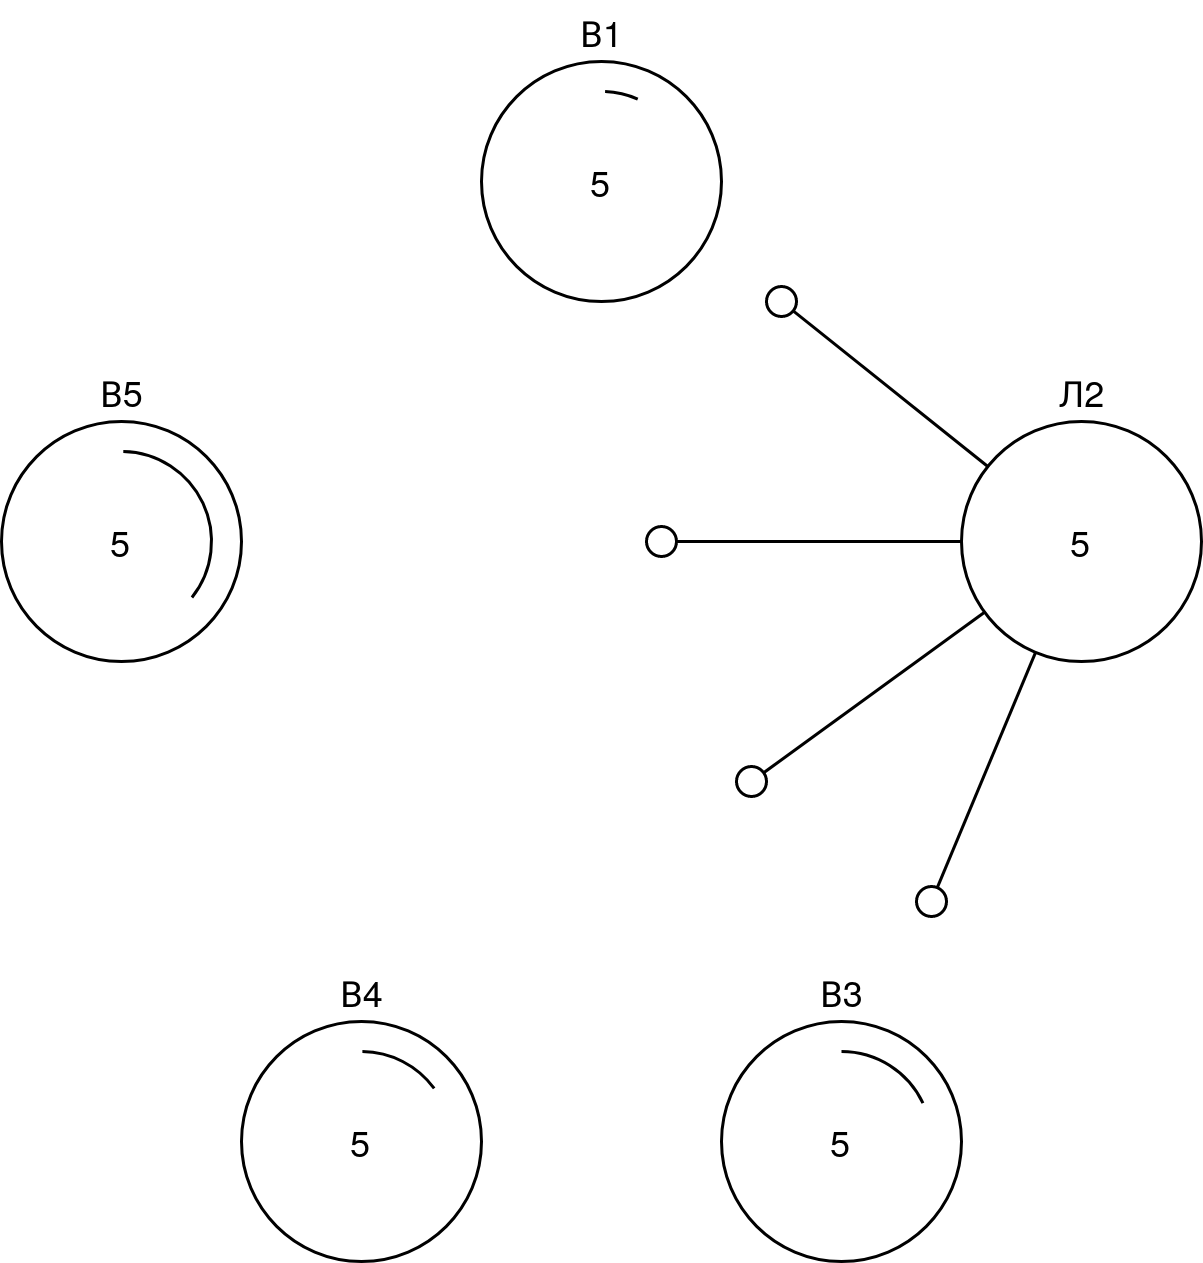
\includegraphics[width=1\linewidth]{src/pics/elec_4.png}} 
\begin{small}
Сервер К2, получив большинство голосов (от В1, В3, В5), становится лидером Л2. Л4, получив сообщение от Л2, отвергает его, так как его номер эпохи больше. Л4, получив от Л2 сообщение,
становится ведомым В4 с эпохой 5, так как обнаруживает, что его номер эпохи устарел \\
\end{small}
\end{minipage}
\caption{}
\label{fig:elec}
\end{figure}

\textbf{Реплицкация журнала}

После того, как лидер был выбран, он начинает обрабатывать запросы клиентов. Каждый запрос клиента содержит команду, которая должна быть выполнена на распределенном конечном автомате. Лидер добавляет команду в свой журнал как новую запись, затем параллельно для каждого сервера вызывает \textit{AppendEntries} чтобы реплицировать эту запись. Когда запись была благополучно реплицированна (эта процедура подробно описывается ниже), лидер применяет команду из новой записи в его конечном автомате и возвращает результат этого вычисления клиенту. Если же какие-то ведомые отказывают, работают медленно, или сетевые пакеты для них теряются, лидер вновь вызывает \textit{AppendEntries} (даже если лидер уже ответил клиенту), пока все ведомые в конечном счете не сохранят эту запись в своих журналах.

Организация журналов показана на \figref{fig:log_1}. Каждая запись журнала хранит команду конечного автомата вместе с номером эпохи, когда запись была получена лидером. Номера эпох в записях журнала используются для обнаружения несоответствий между журналами. Каждая запись журнала также имеет целочисленный индекс, являющийся позицией в журнале.

\begin{figure}[H]
\centering
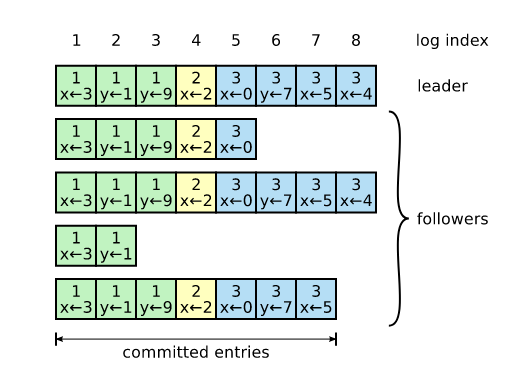
\includegraphics[width=0.95\textwidth]{src/pics/log_1.png}
\caption{Журналы состоят из записей, которые нумеруются последовательно. Каждая запись содержит номер эпохи, в которой он был создан и команду для конечного автомата.}
\label{fig:log_1}
\end{figure}

Лидер решает, когда можно выполнять очередную запись журнала в распределенном конечном автомате; такие применённые записи называются фиксированными. Raft гарантирует, что фиксированные записи не будут потерянны и в конечном итоге будут выполнены на всех доступных конечных узлах. Запись журнала фиксируется лидером, создавшим запись, причем происходит это в тот момент, когда запись успешно реплицируется на большинстве серверов системы. Эта операция также фиксирует все предыдущие записи в журнале лидера, в том числе записи, созданные предыдущими лидерами. Лидер отслеживает наибольший индекс фиксированной записи, и включает этот индекс в вызовы \textit{AppendEntries} (в том числе и при посылке периодических контрольных сообщений), поэтому другие серверы в конечном итоге получают актуальное значение индекса последней записи. После того, как ведомый узнает, что запись журнала была зафиксирована, он применяет эту запись на своем локальном конечном автомате (записи обрабатываются в порядке, соответствующем порядку в журнале).

Raft гарантирует следующие свойства:
\begin{itemize}
\item если две записи в нескольких логах имеют одинаковый индекс и номер эпохи, они содержат одну и ту же команду
\item если две записи в нескольких логах имеют одинаковый индекс и номер эпохи, то все предыдущие команды в этих журналах идентичны
\end{itemize}

Первое свойство следует из того, что лидер создает не более чем одну запись с фиксированным индексом и фиксированным номером эпохи, а все записи никогда не изменяют своего положения в журнале. Второе свойство гарантируется простой проверкой согласованности в реализации процедуры \textit{AppendEntries}. При отправке записи с помощью вызова \textit{AppendEntries}, лидер добавляет индекс и номер эпохи записи, которая непосредственно предшествует новой записи. Если ведомый не находит запись в своем журнале с таким же индексом и эпохой, то он отказывается принимать новую запись. В результате, всякий раз, когда \textit{AppendEntries} успешно завершается, лидер знает, что журнал ведомого идентичен его собственному журналу.

Во время ожидаемой нормальной работы, журналы лидера и ведомых остаются согласованными, поэтому в \textit{AppendEntries} проверка согласованности никогда не закончится неудачно. Однако, в нетривиальных ситуациях, например таких, как отказ лидера, журнал может оказаться в несогласованном состоянии (старый лидер мог не успеть реплицировать все записи в своем журнале). Эти несоответствия могут накапливаться в следствии серии отказов лидеров и ведомых. \figref{fig:log_2} иллюстрирует ситуации, в которых журналы ведомых могут отличаться от нового лидера. Ведомый может не иметь записи, которые присутствуют у лидера (так как лидер не успел реплицировать все записи), он может иметь дополнительные записи, которые не присутствуют у лидера (так как старый лидер начал репликацию записи, но отказал во время выполнения этой операции), так же могут быть записи, которые отсутствуют в обоих серверах. Посторонних записей в журнале может быть несколько.

\vspace{-0.26cm}

\begin{figure}[H]
\centering
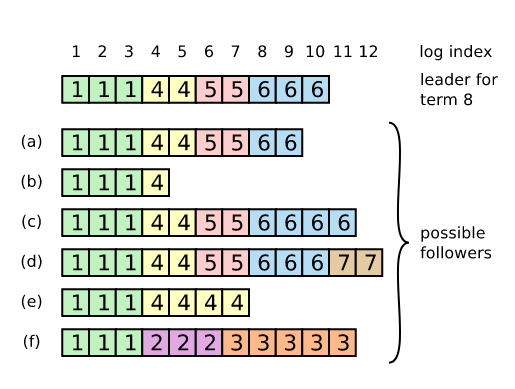
\includegraphics[width=0.9\textwidth]{src/pics/log_2.png}
\caption{Когда лидер (первая строка) побеждает в выборах, то возможны какие-либо из сценариев (а-е) в журналах ведомых. Каждый блок представляет собой одну запись журнала, число внутри блока - номер эпохи соответствующей записи. Ведомый может не иметь некоторых записей (а-б), может иметь дополнительные не зафиксированные записи (в-г), или оба типа дефектов (д-е). Например, сценарий (е) может произойти, если сервер был лидером в эпохе 2 и добавлял несколько записей в свой журнале, но отказал прежде, чем успел зафиксировать какие-либо из них; затем перезапустился, стал лидером на эпоху 3 и добавил несколько записей в свой журнале; прежде, чем какая-либо из записей в эпохе 3 или 2 была зафиксирована, затем лидер снова отказал и не работал в течение нескольких эпох.}
\label{fig:log_2}
\end{figure}

В Raft лидер обеспечивает непротиворечивость, заставляя журналы ведомых дублировать его журнал. Это означает, что конфликтующие записи в журналах ведомых будут перезаписаны с элементами из журнала лидера.

Чтобы согласовать журнал, лидер должен найти последнюю запись в журнале, где два журнала совпадали, стереть все записи в журнале ведомого после этой точки, и отправить ведомому все записи лидера после этой точки. Все эти действия происходят во время проверки согласованности, выполняемой \textit{AppendEntries}. Лидер хранит переменную \textit{next\_index} для каждого ведомого, она хранит индекс записи журнала лидера, которая будет отправлена этому ведомому следующей. Когда сервер впервые становится лидером, он инициализирует все значения \textit{next\_index} номером своей последней записи в своем журнале плюс один. Если журнал ведомого противоречит лидеру, проверка согласованности в процедуре \textit{AppendEntries} откажет при следующем вызове. После отказа, лидер уменьшает \textit{next\_index} и повторяет \textit{AppendEntries}. В конце концов значение \textit{AppendEntries} достигнет точки, где лидер и ведомый имеют идентичные журналы. Когда это произойдет, проверка согласованности \textit{AppendEntries} успешно выполнится, затем процедура удалит конфликтующие записи в журнале ведомого, затем добавит записи из журнала лидера (если таковые имеются). После успешного выполнения процедуры \textit{AppendEntries} журнал ведомого будет согласован с лидером, как минимум до конца текущей эпохи.

С этим механизмом лидеру не нужно предпринимать никаких специальных действий для восстановления журнала, когда он становиться лидером. Ему достаточно начать обычную работу, и журналы автоматически будут согласованны при отказе проверки согласованности процедуры \textit{AppendEntries}. Лидер никогда не перезаписывает или удаляет записи в своем журнале.
Реплицкация журнала позволяет Raft может получать, реплицировать, и фиксировать новые записи, пока большинство из серверов работают

\section{Результаты и тестирование}

Алгоритм, построения распределённой системы на основе имеющегося централизованного сервиса, был разработан и реализован на языке C++ с использованием выше описанного алгоритма решения задачи консенсуса и системы распределённого конечного автомата. 

Созданный алгоритм был применён на существующем сервере лицензий из программного пакета геолого-гидродинамического моделирования тНавигатор. Что позволило создать распределённый сервер лицензий, тем самым значительно повысив его отказоустойчивость и доступность, при некотором замедлении скорости работы.

Тестирование работы созданной распределённой системы проводилось в интернет сети, со средней задержкой передачи сообщений 157мс (миллисекунд).

Далее приведена таблица результатов для изначальной централизованной системы до изменений, а также для кластера распределённой системы, состоящего из 3 и 4 узлов. Измерялось среднее время обработки одного запроса на сервер в первом столбце результатов и среднее время голосования, за которое выбирался новый лидер, в случае отказа текущего во втором столбце. Второй параметр приведён только для распределённой системы и показывает, какой время системы будет недоступна в случае наиболее критичного единичного отказа узла.

\begin{table}[H]
\begin{center}
\begin{tabular}{|c|c|c|}
\hline
Тип системы & \specialcell{Среднее время\\обработки запросов}  & \specialcell{Среднее время\\ голосования}  \\
\hline
Централизованная & 314мс & -  \\
\hline
Кластер из 3 узлов & 614мс & 240мс \\
\hline
Кластер из 4 узлов & 653мс & 404мс \\
\hline
\end{tabular}
\end{center}
\end{table} 

\section{Заключение}

В рамках данной работы была разработана и реализована на языке C++ программа построения распределенной системы из существующего централизованного сервиса на основе алгоритма консенсуса Raft. Что значительно повысило надёжность, отказоустойчивость и добавило возможность масштабирования всей системы.

Реализованная программа была использована для создания распределённой сети из централизованного лицензионного сервера, протестирована и внедрена в программный пакет геолого-гидродинамического моделирования тНавигатор. 


\ifx\undefined\BibEmph\def\BibEmph#1{#1}\else\fi
\ifx\undefined\href\def\href#1#2{#2}\else\fi
\ifx\undefined\url\def\url#1{\texttt{#1}}\else\fi
\ifx\undefined\urlprefix\def\urlprefix{URL: }\else\fi
\ifx\undefined\BibUrl\def\BibUrl#1{\urlprefix\url{#1}}\else\fi
\ifx\undefined\BibUrlDate\long\def\BibUrlDate#1{({%
\cyr\cyrd\cyra\cyrt\cyra\
\cyro\cyrb\cyrr\cyra\cyrshch\cyre\cyrn\cyri\cyrya}: #1)}\else\fi
\ifx\undefined\BibAnnote\long\def\BibAnnote#1{#1}\else\fi

\begin{thebibliography}{1}
\addcontentsline{toc}{section}{\bibname}
\def\selectlanguageifdefined#1{
\expandafter\ifx\csname date#1\endcsname\relax
\else\language\csname l@#1\endcsname\fi}


\bibitem{Theorem_FLP}
\selectlanguageifdefined{english}
\newblock M. Fisher, N. Lynch, M. Paterson
\newblock \em  Impossibility of Distributed Consensus with One Faulty Process\em.
\newblock ACM, Volume 32, Issue 2;
\newblock 1985.

\bibitem{CAP_Theorem}
\selectlanguageifdefined{english}
\newblock S. Gilb ert, N. Lynch, A. Nancy
\newblock \em  Perspectives on the CAP Theorem\em.
\newblock 2012.

\bibitem{Glushkov}
\selectlanguageifdefined{russian}
\newblock Глушков Егор Александрович
\newblock \em Адаптация консенсуса и экосистемы для фреймворка 
Crowdfunding.BGX\em.
\newblock Санкт-Петербургский государственный университет
\newblock Санкт-Петербург.
\newblock 2020.

\bibitem{Blockvhain_review}
\selectlanguageifdefined{english}
\newblock Leila Ismail
\newblock \em A Review of Blockchain Architecture and Consensus Protocols: Use Cases, Challenges, and Solutions\em.
\newblock 2019.

\bibitem{Byzantine_Fault_Tolerance}
\selectlanguageifdefined{english}
\newblock Miguel Castro, Barbara Liskov
\newblock \em Practical Byzantine Fault Tolerance\em.
\newblock 1999.

\bibitem{Raft_search}
\selectlanguageifdefined{english}
\newblock Diego Ongaro, John Ousterhout
\newblock \em In Search of an Understandable Consensus Algorithm\em.
\newblock 2014.

\end{thebibliography}
\bibliographystyle{gost705}


\end{document}